\documentclass[xindy,rascunho]{fei}
\usepackage[utf8]{inputenc}
%\usepackage{minted,multicol}
%\hypersetup{pdftitle={Reconhecimento de Padrões em Conversas utilizando Redes Complexas},
%pdfauthor={Gabriel Lett Viviani, Gabriel Tamassia Martinez, Gabriel Reis Dias e Ítalo Cuzziol Ferreira},
%pdfsubject={Reconhecimento de Padrões},
%pdfkeywords={Redes Complexas, Reconhecimento de Padrões}
%}
\author{Gabriel Lett Viviani \and Gabriel Tamassia Martinez \and Gabriel Reis Dias \and Ítalo Cuzziol Ferreira}
\title{Reconhecimento de Padrões em Conversas utilizando Redes Complexas}
%\subtitulo{subtítulo}
\cidade{São Bernardo do Campo}
\instituicao{Centro Universitário da FEI}

\begin{document}

\maketitle

\begin{folhaderosto}
Trabalho de Conclusão de Curso, apresentado no Centro Universitário da FEI, como parte dos requisitos necessários para obtenção do título de Bacharel em Ciência da Computação, orientado pelo professor Rodrigo Filev Maia.
\end{folhaderosto}

%\fichacatalografica
%\folhadeaprovacao
\dedicatoria{A quem eu quero dedicar o texto.}
\begin{agradecimentos}
Lorem ipsum dolor sit amet, consectetur adipiscing elit. Aenean quam turpis, ullamcorper quis laoreet ac, malesuada sed mi. Quisque orci nunc, placerat quis mauris vel, luctus dictum tellus. Ut aliquam dui nunc, quis commodo justo mattis aliquam. Nam congue libero nec dui auctor pharetra. Sed sit amet justo sodales, elementum massa quis, luctus ipsum. Ut et libero mattis, rhoncus nisi vitae, facilisis sapien. Aliquam erat volutpat. Mauris eget libero egestas, ullamcorper leo quis, convallis libero. Lorem ipsum dolor sit amet, consectetur adipiscing elit.

Sed a odio porttitor, lacinia libero vel, egestas sem. Donec accumsan tellus nec enim porttitor, id rhoncus neque dignissim. Vestibulum sollicitudin turpis sed ligula tincidunt iaculis. Vestibulum condimentum libero erat, laoreet placerat elit ullamcorper a. Nam consectetur euismod risus. Duis quis ultricies velit, ut volutpat augue. Nam ligula sapien, interdum id leo vitae, porta volutpat velit. Class aptent taciti sociosqu ad litora torquent per conubia nostra, per inceptos himenaeos. Vivamus sit amet libero varius, consequat ipsum ac, placerat velit.

Nunc molestie nunc ac lorem dictum, sit amet placerat tellus congue. In sit amet dolor sed leo lobortis malesuada. Curabitur sit amet tristique urna. Vestibulum sollicitudin pellentesque aliquam. Sed pellentesque enim in lacus sodales laoreet. Suspendisse massa magna, fermentum at massa vitae, fermentum posuere dui. Interdum et malesuada fames ac ante ipsum primis in faucibus. Pellentesque porttitor mauris adipiscing dolor semper condimentum. Donec in nibh sapien. Cras vestibulum venenatis nisl ultrices feugiat. Donec a neque eu odio vehicula rutrum quis eu nisl. Curabitur mauris diam, sollicitudin egestas condimentum a, faucibus non felis. Duis scelerisque augue sed turpis lobortis accumsan.

Class aptent taciti sociosqu ad litora torquent per conubia nostra, per inceptos himenaeos. Duis ut dolor erat. Fusce adipiscing interdum eros, in ultrices orci auctor at. Mauris ac ante orci. In nec mauris arcu. In pulvinar tortor a felis interdum pretium. Donec tristique laoreet sollicitudin. Proin erat metus, blandit sed cursus eget, faucibus id nunc. Donec id nisi non mauris tempor tincidunt. Fusce venenatis pulvinar enim. Fusce sit amet tortor nec magna feugiat pharetra ac nec nibh. Praesent non nisi lacus. Class aptent taciti sociosqu ad litora torquent per conubia nostra, per inceptos himenaeos. Vestibulum rutrum varius velit, id iaculis ante vestibulum quis. Aenean bibendum sit amet quam ornare mollis. Suspendisse sollicitudin fringilla felis in venenatis.

Vivamus vel erat erat. Integer venenatis nisl velit, vel commodo lectus condimentum ac. Aliquam id magna at tellus sagittis tempus id quis ante. Maecenas bibendum ipsum nec urna condimentum mollis. In venenatis eget nunc ac adipiscing. Vivamus faucibus vel orci mattis egestas. In hac habitasse platea dictumst. Nulla faucibus neque eu fermentum luctus. Duis ipsum nunc, congue vel justo nec, faucibus iaculis erat. Integer sit amet augue nec enim blandit placerat. Sed bibendum feugiat eros.
\end{agradecimentos}
\epigrafe{A good scientist is a person with original ideas. A good engineer is a person who makes a design that works with as few original ideas as possible. There are no prima donnas in engineering.}{Freeman Dyson \nocite{dyson_disturbing_1979}}

\begin{resumo}
Com o avanço da tecnologia e maior facilidade de acesso à internet para toda população, é normal que os pais fiquem preocupados com a segurança de seus filhos que estão navegando na rede. Hoje tem-se diversos meios de entretenimento, como jogar online, assistir a vídeos engraçados e poder conversar com amigos que estão distantes através de mensagens de texto ou por voz, como viabiliza o Skype, Axon e outros aplicativos. Mas também é possível se utilizar destes meios para um propósito malicioso, como acontece em salas de bate papo onde se tem uma certa liberdade para poder introduzir o assunto que desejar, visto que é muito complexo modelar um analisador de textos computacional – sendo esta uma tarefa que cabe ao ser humano realizar – e assim propiciando ataques de pedófilos, por exemplo.
 Visto a necessidade de se reconhecer um padrão dado um texto qualquer almejando a identificação de um ataque, a proposta dessa tese é analisar uma base de dados que contenha ataques de pedófilos, detectar um padrão e constatar se um padrão similar acontece em redes livres de ataques, que aqui serão chamadas de “base ordinária” ou “base inocente” .
 
\palavraschave{Redes Complexas. Detecção de Comunidades. Reconhecimento de Padrões.}
\end{resumo}

\begin{abstract}
Lorem ipsum dolor sit amet, consectetur adipiscing elit. Aenean quam turpis, ullamcorper quis laoreet ac, malesuada sed mi. Quisque orci nunc, placerat quis mauris vel, luctus dictum tellus. Ut aliquam dui nunc, quis commodo justo mattis aliquam. Nam congue libero nec dui auctor pharetra. Sed sit amet justo sodales, elementum massa quis, luctus ipsum. Ut et libero mattis, rhoncus nisi vitae, facilisis sapien. Aliquam erat volutpat. Mauris eget libero egestas, ullamcorper leo quis, convallis libero. Lorem ipsum dolor sit amet, consectetur adipiscing elit.

Sed a odio porttitor, lacinia libero vel, egestas sem. Donec accumsan tellus nec enim porttitor, id rhoncus neque dignissim. Vestibulum sollicitudin turpis sed ligula tincidunt iaculis. Vestibulum condimentum libero erat, laoreet placerat elit ullamcorper a. Nam consectetur euismod risus. Duis quis ultricies velit, ut volutpat augue. Nam ligula sapien, interdum id leo vitae, porta volutpat velit. Class aptent taciti sociosqu ad litora torquent per conubia nostra, per inceptos himenaeos. Vivamus sit amet libero varius, consequat ipsum ac, placerat velit.

Nunc molestie nunc ac lorem dictum, sit amet placerat tellus congue. In sit amet dolor sed leo lobortis malesuada. Curabitur sit amet tristique urna. Vestibulum sollicitudin pellentesque aliquam. Sed pellentesque enim in lacus sodales laoreet. Suspendisse massa magna, fermentum at massa vitae, fermentum posuere dui. Interdum et malesuada fames ac ante ipsum primis in faucibus. Pellentesque porttitor mauris adipiscing dolor semper condimentum. Donec in nibh sapien. Cras vestibulum venenatis nisl ultrices feugiat. Donec a neque eu odio vehicula rutrum quis eu nisl. Curabitur mauris diam, sollicitudin egestas condimentum a, faucibus non felis. Duis scelerisque augue sed turpis lobortis accumsan.

Class aptent taciti sociosqu ad litora torquent per conubia nostra, per inceptos himenaeos. Duis ut dolor erat. Fusce adipiscing interdum eros, in ultrices orci auctor at. Mauris ac ante orci. In nec mauris arcu. In pulvinar tortor a felis interdum pretium. Donec tristique laoreet sollicitudin. Proin erat metus, blandit sed cursus eget, faucibus id nunc. Donec id nisi non mauris tempor tincidunt. Fusce venenatis pulvinar enim. Fusce sit amet tortor nec magna feugiat pharetra ac nec nibh. Praesent non nisi lacus. Class aptent taciti sociosqu ad litora torquent per conubia nostra, per inceptos himenaeos. Vestibulum rutrum varius velit, id iaculis ante vestibulum quis. Aenean bibendum sit amet quam ornare mollis. Suspendisse sollicitudin fringilla felis in venenatis.

Vivamus vel erat erat. Integer venenatis nisl velit, vel commodo lectus condimentum ac. Aliquam id magna at tellus sagittis tempus id quis ante. Maecenas bibendum ipsum nec urna condimentum mollis. In venenatis eget nunc ac adipiscing. Vivamus faucibus vel orci mattis egestas. In hac habitasse platea dictumst. Nulla faucibus neque eu fermentum luctus. Duis ipsum nunc, congue vel justo nec, faucibus iaculis erat. Integer sit amet augue nec enim blandit placerat. Sed bibendum feugiat eros.
\keywords{Keywords. Go. Here.}
\end{abstract}

%\listoffigures
%\listoftables
%\listofalgorithms
%\glsaddall
%\printglossaries
\tableofcontents

\chapter{Introdução}

O abuso sexual contra crianças é um problema que vem ganhando visibilidade nos últimos anos, devido à popularização da internet, que facilita a realização de pesquisas escolares, socialização entre amigos e divertimento. Com isso muitos pedófilos veem uma oportunidade para buscar suas vítimas na internet.

A cada ano, mais de 3 milhões de relatos de abuso de crianças são feitos apenas nos Estados Unidos [http://www.childhelp.org/pages/statistics, 19/04/2014 18:00]. Este é um problema que se agravou com o anonimato que internet propicia. Por isso a criação de ferramentas automáticas capazes de identificar pedófilos na rede, de forma massiva, se tornou uma necessidade.

Propõe-se apresentar nesse trabalho uma solução que seja capaz de reconhecer um indivíduo malicioso através de técnicas de modelagem de dados e análise textual. Esse tipo de problema pode ser estruturado utilizando o conceito de redes complexas para modelagem das bases analisadas e processamento de textos para extrair e pré-processar os dados necessários a serem inseridos na rede.

Diego Raphael Amancio apresentou um trabalho (>N<) com muitas técnicas que serão utilizadas nesse trabalho. No trabalho ele utilizou redes complexas para modelar o texto, estudou certas métricas topológicas na aplicação de processamento de línguas naturais, mostrou que a maioria das medidas de rede depende de fatores sintáticos, e medidas de intermitência são mais sensíveis à semântica, todos conceitos uteis a esse trabalho.

O conceito de redes complexas foi escolhido para analisar este problema porque acreditamos que sua estrutura se assemelha à de redes reais, como as de sistemas sociais e sistemas biológicos, por exemplo [STROGGATZ? CITAÇÃO, 2011], no que diz respeito à presença e detecção de comunidades. Isso porque a detecção da comunidade de palavras à qual um pedófilo pertence ajuda na identificação de um possível agressor. Além disso, outros trabalhos (>N<) aplicando técnicas como Support Vector Machines (SVM) já estudaram a identificação de pedófilos utilizando aprendizado de máquina.

O processamento de textos será utilizado para analisar as bases de conversas e estruturar as palavras para posterior formação da rede, e.g. filtrando abreviações e sinais de pontuação.

\section{Objetivos}

O objetivo principal é a construção de um modelo computacional que permita a verificação da existência de padrões comportamentais de pedófilos em uma base, utilizando algoritmos de detecção de comunidades em redes complexas e processamento de textos.

\section{Organização do Trabalho}

No capítulo 1 é apresentada a introdução do problema a ser tratado e sua possível solução. O capítulo 2 trata do embasamento teórico referente a redes complexas. No capítulo 3 é apresentado conceitos de processamento de textos. O capítulo 4 apresenta as estratégias que serão utilizadas nessa tese. O capítulo 5 descreve as considerações finais sobre o assunto.

\chapter{Redes Complexas}

O estudo de redes está presente em diversas áreas da ciência, da sociologia à neurobiologia e física estatística. Alguns estudos empíricos com redes foram feitos, esclarecendo questões topológicas de redes alimentares, redes celulares e metabólicas, e redes de computadores, só para citar alguns exemplos [STROGATZ, 2001, NATURE].

Uma rede (ou grafo) pode ser definida matematicamente como $ G= (V,E) $, aonde $V$ é o conjunto de vértices e $E$ é o conjunto de arestas que fazem parte da rede. Ela pode ainda ser direcionada, quando as arestas possuem uma direção. A conectividade entre os vértices é representada por uma matriz de adjacência simétrica $A$, aonde cada elemento $a_ij$ da matriz indica se o vértice $v_i$ está conectado ao vértice $v_j$ quando $a_ij=1$.

Redes complexas são redes com características específicas, como, por exemplo, a estrutura mundo pequeno (ou small-world) (ver Figura 2.1) quando modelando sistemas reais [REF4, AMANCIO]. Algumas das complicações de redes complexas são: complexidade estrutural, evolução da rede, diversidade de conexões, complexidade dinâmica, diversidade de nós e meta-complicações [STROGATZ, 2001, NATURE].

As estruturas de redes complexas podem ser úteis nos estudos de diversos ramos, como, por exemplo, na Biologia, ao verificar como uma doença se propaga entre os indivíduos, permitindo fazer uma análise, tomar alguma providência e evitar uma possível epidemia; ou até mesmo a Internet, verificando como estão interligadas as redes, se estão assegurando a sua disponibilidade, se evitam redundâncias desnecessárias, ou verificando qual o menor caminho até o destino.

\section{Modelos de Redes Complexas}

Os principais modelos topológicos de redes complexas são as redes aleatórias, redes mundo pequeno (small-world) e redes livre-de-escala (scale-free).

\subsection{Redes Aleatórias}

As redes aleatórias são redes aonde todas as ligações feitas são aleatórias. Imagine que uma rede tenha $n>>1$ vértices e que todas as m ligações dessa rede foram feitas de forma aleatória. Erdös e Rényi estudaram esse modelo e analisaram alguns comportamentos dela. Quando $m$ é muito pequeno, a rede tende a ser fragmentada em pequenos clusters de vértices, também chamados de componentes. Aumentando $m$, os vértices isolados tendem a se ligarem com componentes já existentes, e depois os componentes começam a se interligarem. Quando $m>n/2$ os vértices do maior componente da rede estão ligados entre si por caminhos curtos [STROGATZ, 2001, NATURE].

\begin{figure}
\centering
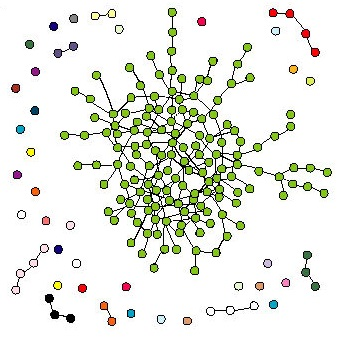
\includegraphics[width=0.7\linewidth]{./Imagens_Monografia/410268ac2(RedeAleatoria).jpg}
\caption{Uma rede aleatória com 200 vértices e 193 arestas. Nota-se a presença de um grande componente, alguns vértices e pequenos componentes na parte externa e a ausência de hubs [Imagem de STROGATZ, 2001, NATURE]}
\label{fig:RedeAleatoria}
\end{figure}


\subsection{Redes de Mundo Pequeno}

Já as redes mundo pequeno, estudas por Watts e Strogatz, são redes intermediárias entre as redes regulares e as rede aleatórias. Nesse modelo, uma rede regular tem suas conexões trocadas por conexões aleatórias com uma probabilidade entre 0 e 1. A rede resultante, mesmo com um pequeno número de reconexões, transforma a rede em um "pequeno mundo", com curtos caminhos entre quaisquer dois vértices. Além disso, essa rede é muito aglomerada: se $A$ está ligado a $B$ e $B$ está ligado a $C$, há uma probabilidade maior de que $A$ esteja ligado a $C$ [STROGATZ, 2001, NATURE].

\begin{figure}
\centering
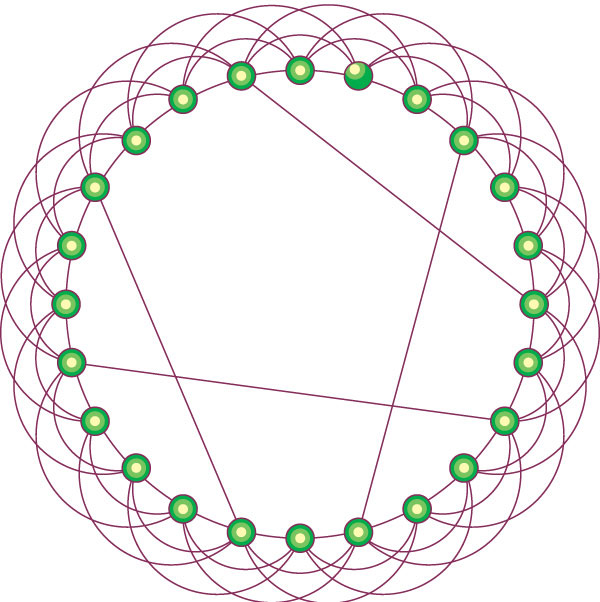
\includegraphics[width=0.7\linewidth]{./Imagens_Monografia/410268ad2(Small-world_Strongatz_2001).jpg}
\caption{Representação de uma rede mundo-pequeno com topologia em anel. Essa rede possui 24 nós e cada nó está conectado a seus três vizinhos mais próximos. 
Fonte: [Imagem de STROGATZ, 2001, NATURE].}
\label{fig:RedeMundoPequeno}
\end{figure}

\subsection{Redes Livre de Escala}

Por fim, as redes livre de escala são redes que também se encontram entre redes regulares e redes aleatórias. A principal característica desse modelo (também chamado de modelo Barabási-Albert) são os hubs, vértices que são bem conectados a outros vértices, ou seja, possuem um alto grau de vértice (ver item 2.1.1). O estudo de Albert, Barabási e Jeong sobre esse modelo, sugere que o crescimento das redes é baseado em regras de conexões preferenciais. Ou seja, alguns vértices são “preferidos” para se conectarem a outros vértices [STROGATZ, 2001, NATURE][AMANCIO, 2013].

\begin{figure}
\centering
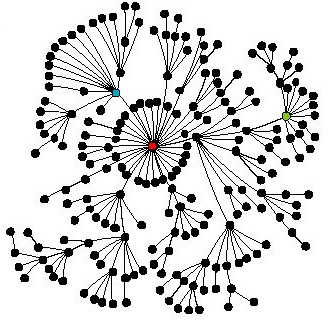
\includegraphics[width=0.7\linewidth]{./Imagens_Monografia/410268ac2(RedeLivreDeEscala).jpg}
\caption{Um grafo livre de escala, construído com 200 vértices e 199 arestas. A construção deu preferencia aos nós com maior grau de vértice para ligação com novos nós. Assim, nós com maior grau de vértice tenderam a ficar com mais ligações e nós com menor grau de vértice tenderam a ficar com menos ligações. Fonte: [Imagem de STROGATZ, 2001, NATURE].}
\label{fig:RedeLivreDeEscala}
\end{figure}

\section{Métricas de Redes Complexas}

As redes complexas apresentam diferentes topologias, como pode ser observado quando se comparam redes sociais com tecnológicas (como a Internet) ou biológicas – cada uma possui uma arquitetura distinta [tese.pdf et al].  Surgiu à necessidade de quantificar essas estruturas de ligações através de medidas, que têm sido desenvolvidas para analisar, caracterizar, classificar e modelar as redes complexas. Existem diversas medidas, mas apenas algumas serão utilizadas nesse trabalho.

\subsection{Grau de um vértice}
Considerada uma das mais simples medidas de se calcular, o grau de um vértice define se ele é relevante (alto) ou de pouca importância (baixo) [Amancio 2013]. O grau corresponde ao número de arestas que incidem sobre um nó V, sendo calculado através da fórmula abaixo:
\begin{equation} \label{eq:GrauVertice}
k = \sum_{j = i}^{M}a_{ij} = \sum_{i=1}^{M}a_{ij}
\end{equation}

\subsection{Betweenness}
Outra métrica que tem o conceito de centralidade mas é diferente do grau se denomina betweenness. Os vértices que possuírem valores altos podem ser considerados como nós com alta influência na rede [Amancio 2013]. 

No contexto de reconhecimento de padrões abordado nessa tese,  palavras que aparecem muitas vezes tendem a possui um valor do betweenness elevado. Com essa informação, pode-se dizer que uma mesma palavra que apareça frequentemente na rede tenha contextos distintos, desempenhando um papel de ponto de articulação entre comunidades [Amancio 2013].

Para essa medida, [Amancio 2013] sugeriu calculá-la de forma normalizada, de modo a eliminar correlações com outras medidas (por exemplo o grau $k$), através da equação a seguir:

\begin{equation} \label{eq:Betweenness}
B_i = \frac{1}{M^2} \sum_{s=1}^{M}\sum_{t=1}^{M}\frac{n_{sit}}{n_{st}}
\end{equation}

Onde $B_i$ é valor da métrica betweenness, $n_sit$ é o número de caminhos mínimos de um vértice $s$ ligados a outro vértice $t$ passando pelo ponto $i$, enquanto $n_st$ é o caminho mínimos sem passar pelo vértice $i$. Assim o valor de $B$ varia entre [0,1].

\subsection{Coeficiente de Aglomaração}
O coeficiente de aglomeração (clustering coefficient) começa a olhar mais os vizinhos (arestas) ao invés da centralidade do vértice. A ideia é medir a razão entre o número de arestas entre os vizinhos de um vértice v e o número máximo possível de arestas entre esses vizinhos [tese.pdf et al]. Por definição, se o vértice possuir menos de dois vizinhos, seu coeficiente de aglomeração é igual a zero [Amancio 2013].

Espera-se, então, que as palavras com altos valores desse coeficiente possuam diversos vizinhos conectados entre si, e que o contrário também se aplique – nós cujos vizinhos não estejam se relacionando entre si apresentem valores mais baixos [Amancio 2013].

O cálculo se dá através da fórmula abaixo:

\begin{equation} \label{eq:CoefAglomeracao}
C = \frac{2e_i}{k_i(k_i - 1)}
\end{equation}

Onde $C$ é o valor do coeficiente de aglomeração, $e_i$ é o número de arestas entre os vizinhos (excluindo as arestas que estão ligadas ao vértice $i$) [tese.pdf].

\subsection{Distribuição de Pesos }
A distribuição de pesos permite verificar a frequência que cada peso aparece na rede. A partir da distribuição de pesos, em conjunto com a topologia da rede, possibilita extrair algumas informações como a entropia da distribuição. Alta entropia indica concentração de informação, já baixa entropia indica uma rede mais distribuída em vários conjuntos.

A extração da distribuição de pesos pode ser realizada determinando inicialmente o número de discretizações a serem utilizadas, de acordo com os possíveis valores da rede. Após esta definição, uma varredura na rede é realizada, identificando em qual faixa se encontra cada nó percorrido. 

Ao final teremos armazenado a quantidade de elementos em cada faixa de peso, gerando-se assim um histograma de valores.
O algoritmo é proporcional a quantidade de arestas, podendo ser em seu pior caso $O(N)^2$, ao percorrer todas as arestas da rede [Guilherme].

\subsection{Densidade de Conexão Média}
A densidade de conexão média ($K_{den}$) compara uma rede qualquer a uma mesma rede com a mesma quantidade de arestas completa. Esta medida varia de 0 a 1 e está relacionada a completude do grafo.

A seguinte equação é utilizada para calcular ($K_{den}$) para redes não dirigidas:

\begin{equation} \label{eq:DensidadeNaoDirigida}
K_{den} = 2 \cdot \frac{|E|}{n^2 - n}
\end{equation}

Já para redes dirigidas, utilizamos a seguinte equação:

\begin{equation} \label{eq:DensidadeDirigida}
K_{den} = \frac{|E|}{n^2 - n}
\end{equation}

onde $|E|$ é o conjunto de células da matriz de pesos, sendo que o peso deve ser superior a 0. 
Caso o valor das equações seja baixo, estamos lidando com uma rede considerada esparsa. Caso contrário, a rede pode ser considerada densa, pois contém muitas arestas [Guilherme].

\subsection{Índice de Semelhança de Conexão}
O índice de semelhança de conexão $p_{i,j}$ (para $i \neq j$) mede o quanto as conexões do nó $i$ é semelhante as conexões do nó $j$. O calculo é efetuado através da soma da quantidade de nós semelhantes de $i$ e $j$, sendo os nós semelhantes os nós de $i$ que conectam aos mesmos nós $j$.

Supondo-se que $A$ é o conjunto de nós conectados a $i$ e $B$ o conjunto de nós conectados a $j$, o índice de semelhança de conexão $p_{i,j}$ é obtido através da seguinte equação:

\begin{equation} \label{eq:IndiceSemelhanca}
p_{i,j} = \frac{|A \bigcap B|}{|A \bigcup B|}
\end{equation}

[GUILHERME] propõe através deste índice, comparar dois nós através de suas conexões e identificar possíveis clusterizações baseadas nesta medida.

\section{Comunidades}
Em redes aleatórias quase todos os vértices têm um mesmo grau, o que as torna praticamente homogêneas. Redes reais apresentam uma distribuição de arestas diferente, mais parecida com a das redes livres de escala, com alguns vértices com muitas arestas conectadas e muitos com poucas arestas os conectando. Essa característica é conhecida como comunidade, cluster ou módulo [Community Detection in Graphs, Santo Fortunato].

Comunidades não têm uma definição global. Uma diretriz para a definição de comunidades é a de que existem mais arestas conectando os vértices dentro de uma comunidade do que arestas conectando os vértices da comunidade a outras comunidades [Community Detection in Graphs, Santo Fortunato].

Vértices dentro de uma mesma comunidade tendem a apresentar características semelhantes e/ou ter papéis semelhantes na rede em questão [Community Detection in Graphs, Santo Fortunato].

\begin{figure}
\centering
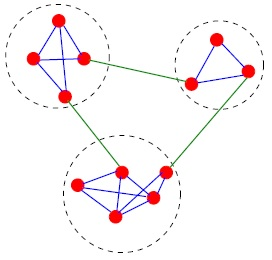
\includegraphics[width=0.7\linewidth]{./Imagens_Monografia/Community_Detection_in_Graphs_-_Santo_Fortunato(Representacao_Comunidades).jpg}
\caption{Uma rede pequena com três comunidades (circuladas pelos tracejados). 
Fonte: [Community Detection in Graphs, Santo Fortunato]}
\label{fig:Comunidade}
\end{figure}

A identificação de comunidades pode ser usada para diversos fins. Por exemplo, é possível detectar pessoas que pertençam a um mesmo grupo de relacionamento quando mapea-se relações entre as pessoas, ou identifica-se um grupo de clientes que possuam interesses parecidos quando mapeando as relações entre clientes e compras [Community Detection in Graphs, Santo Fortunato].

\subsection{Métodos de Detecção de Comunidades}
Existem diversos métodos para detectar comunidades em um grafo, como os tradicionais, os baseados em modularidade, os baseados em inferência estatística, entre outros. Nesse tópico serão abordados alguns desses métodos.

\subsubsection{Partição de Grafo}
Na partição de grafo procura-se dividir os vértices do grafo em $g$ grupos de tamanhos pré-estabelecidos, com o menor número possível de arestas ligando duas comunidades. Nesse método para solução é necessário informar o número de comunidades que se procuram, assim como o tamanho das comunidades. Esse método é usado em partição de circuitos, computação paralela, entre outros [Community Detection in Graphs, Santo Fortunato].

\begin{figure}
\centering
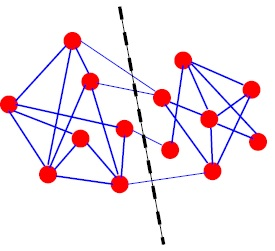
\includegraphics[width=0.7\linewidth]{./Imagens_Monografia/Community_Detection_in_Graphs_-_Santo_Fortunato(Particionamento_Grafos).jpg}
\caption{Partição de grafo com duas comunidades de tamanho igual. A linha tracejada representa a separação entre as comunidades com uma quantidade mínima de arestas interligando-as. 
Fonte: [Community Detection in Graphs, Santo Fortunato]}
\label{fig:ParticaoDeGrafo}
\end{figure}

\subsubsection{Agrupamento Hierárquico}
Muitas vezes não há informação sobre a quantidade de comunidades que existem no grafo, o que faz a aplicação do método de Partição de Grafo de pouca ajuda. Métodos como o Agrupamento Hierárquico visam agrupar vértices em uma estrutura de níveis, com comunidades menores dentro de comunidades maiores, e essas comunidades maiores dentro de outra maior ainda, e assim por diante. Redes sociológicas, por exemplo, frequentemente são estruturadas dessa maneira [Community Detection in Graphs, Santo Fortunato].

Nesse método, a primeira coisa a se definir é a medida de similaridade entre os nós. Com essa medida em mãos, deve-se calcular a similaridade entre dois nós, não se importando se estão conectados ou não. No final do processo, a matriz de similaridade é utilizada para agrupar vértices com alto grau de similaridade. Existem duas categorias de técnicas para realizar esse agrupamento [Community Detection in Graphs, Santo Fortunato]:
\begin{enumerate}
	\item Algoritmos de Aglomeração, aonde comunidades são agrupadas, se sua similaridade é alta o bastante;
	\item Algoritmos Divisivos, aonde comunidades são divididas, através da remoção de arestas, se seus nós apresentam similaridades suficientemente baixas.
\end{enumerate}

\chapter{Processamento de Textos}
Nesse capítulo será descrito como as palavras da base de dados serão tratadas para viabilizar a modelagem da rede complexa. 

\section{Pré-Processamento de Textos}
Nessa fase as frases passam por processos que visam transformar toda a base de dados composta por texto em uma rede complexa. Para isso, será aplicado alguns passos que Diego Raphael Amancio utilizou em sua tese de “Classificação de Texto com Redes Complexas”, onde ele sugere retirar sinais de pontuação e palavras de pouca relevância, tratadas como stopwords (preposições, por exemplo). 

Após a filtragem das stopwords, Amancio explica que faz um processo de lematização das palavras que restaram, como transformar palavras que estão no plural em sua devida forma no singular e verbos que estão conjugados em sua forma original no infinitivo. E com isso, todas as palavras que referenciam um mesmo conceito estão associados a um mesmo vértice.

Com isso, a nova base estará pronta para ser processada e assim iniciar a modelagem da rede complexa.

\subsection{Part-of-speech tagging}

\section{Construção da rede escrita}
Depois da fase de pré-processamento de textos, é possível fazer a contagem de palavras distintas que a base possui, e consequentemente definir quantos nós a rede terá. Para cada par de palavras, existe uma aresta direcionada de um nó a outro [arq0054.pdf]. Existe três tipos de redes predominantes na modelagem da linguagem como redes complexas: co-ocorrência, sintática e semântica [Amancio 2013].

\subsection{Redes de co-ocorrência}
Escrever aqui senhores, Amancio tem uma descrição dessas 3 redes, e mais a tese do Guilherme.

\subsection{Redes sintáticas}
Amancio.

\subsection{Redes semânticas}
Amancio.

\section{Medidas Estatísticas}
Amancio (medidas básicas) e arq0054.pdf (capitulo 3). Provavelmente será pequeno, não repetir o que foi dito no capítulo 2.1

\section{Entropia}
Amancio.

\section{Intermitência de palavras}
Verificar com o Filev (Amancio).

\chapter{Estratégia}
Para atingir o objetivo, será utilizado uma abordagem baseada em redes complexas. A estratégia de solução é estruturada em duas etapas principais: a primeira de construção das redes, e a segunda de análise, que visa estudar quais características podem ser retiradas de cada rede construida. As redes utilizadas serão direcionadas.

Na primeira etapa serão construídas duas redes, uma baseada em um conjunto de conversas contendo apenas pedófilos e outra baseada em um conjunto de conversas contendo apenas conversas ordinárias. A base de conversas contendo apenas pedófilos será retirada da página do PJ (www.perverted-justice.com) que assegura que os dados em suas bases são de diálogos entre um pedófilo e uma criança. A base de conversas ordinárias não conterá diálogos entre pedófilos e as vítimas, e será extraída da base do PAN2012 (disponível para download em http://www.uni-weimar.de/medien/webis/research/events/pan-12/pan12-web/author-identification.html). Contudo, há uma mescla de conversas na base do PAN2012, ou seja, há tanto conversas ordinárias quanto a de pedofilia. Será selecionado apenas as conversas “limpas”, sendo necessário fazer uma análise e assim rotulá-las, e selecionar apenas as que forem rotuladas como “ordinárias”. 

O parser terá a função de ler as tags HTML, escritas em um determinados padrão, após esta leitura, ele armazena as conversas em objetos intermediários em memória. Os objetos são, então, persistidos na base de dados orientada a grafos, para que seja possível sua futura verificação, extração de métricas e suas características.
A construção das redes será criteriosa em relação às palavras que entrarão na rede. A princípio, sinais de pontuação e algumas palavras com pouco conteúdo semântico (chamadas stopwords) serão excluídos da rede.
Na segunda etapa, com as bases estruturadas, inicia-se um trabalho de levantamento de dados, como identificar as características que a rede de pedófilos tem, se as mesmas informações aparecem na rede ordinária, comparar as métricas entre essas informações, e identificar padrões que digam se, dada uma rede x, esta é classificada como ordinária ou como de pedófilos.

\begin{figure}
\centering
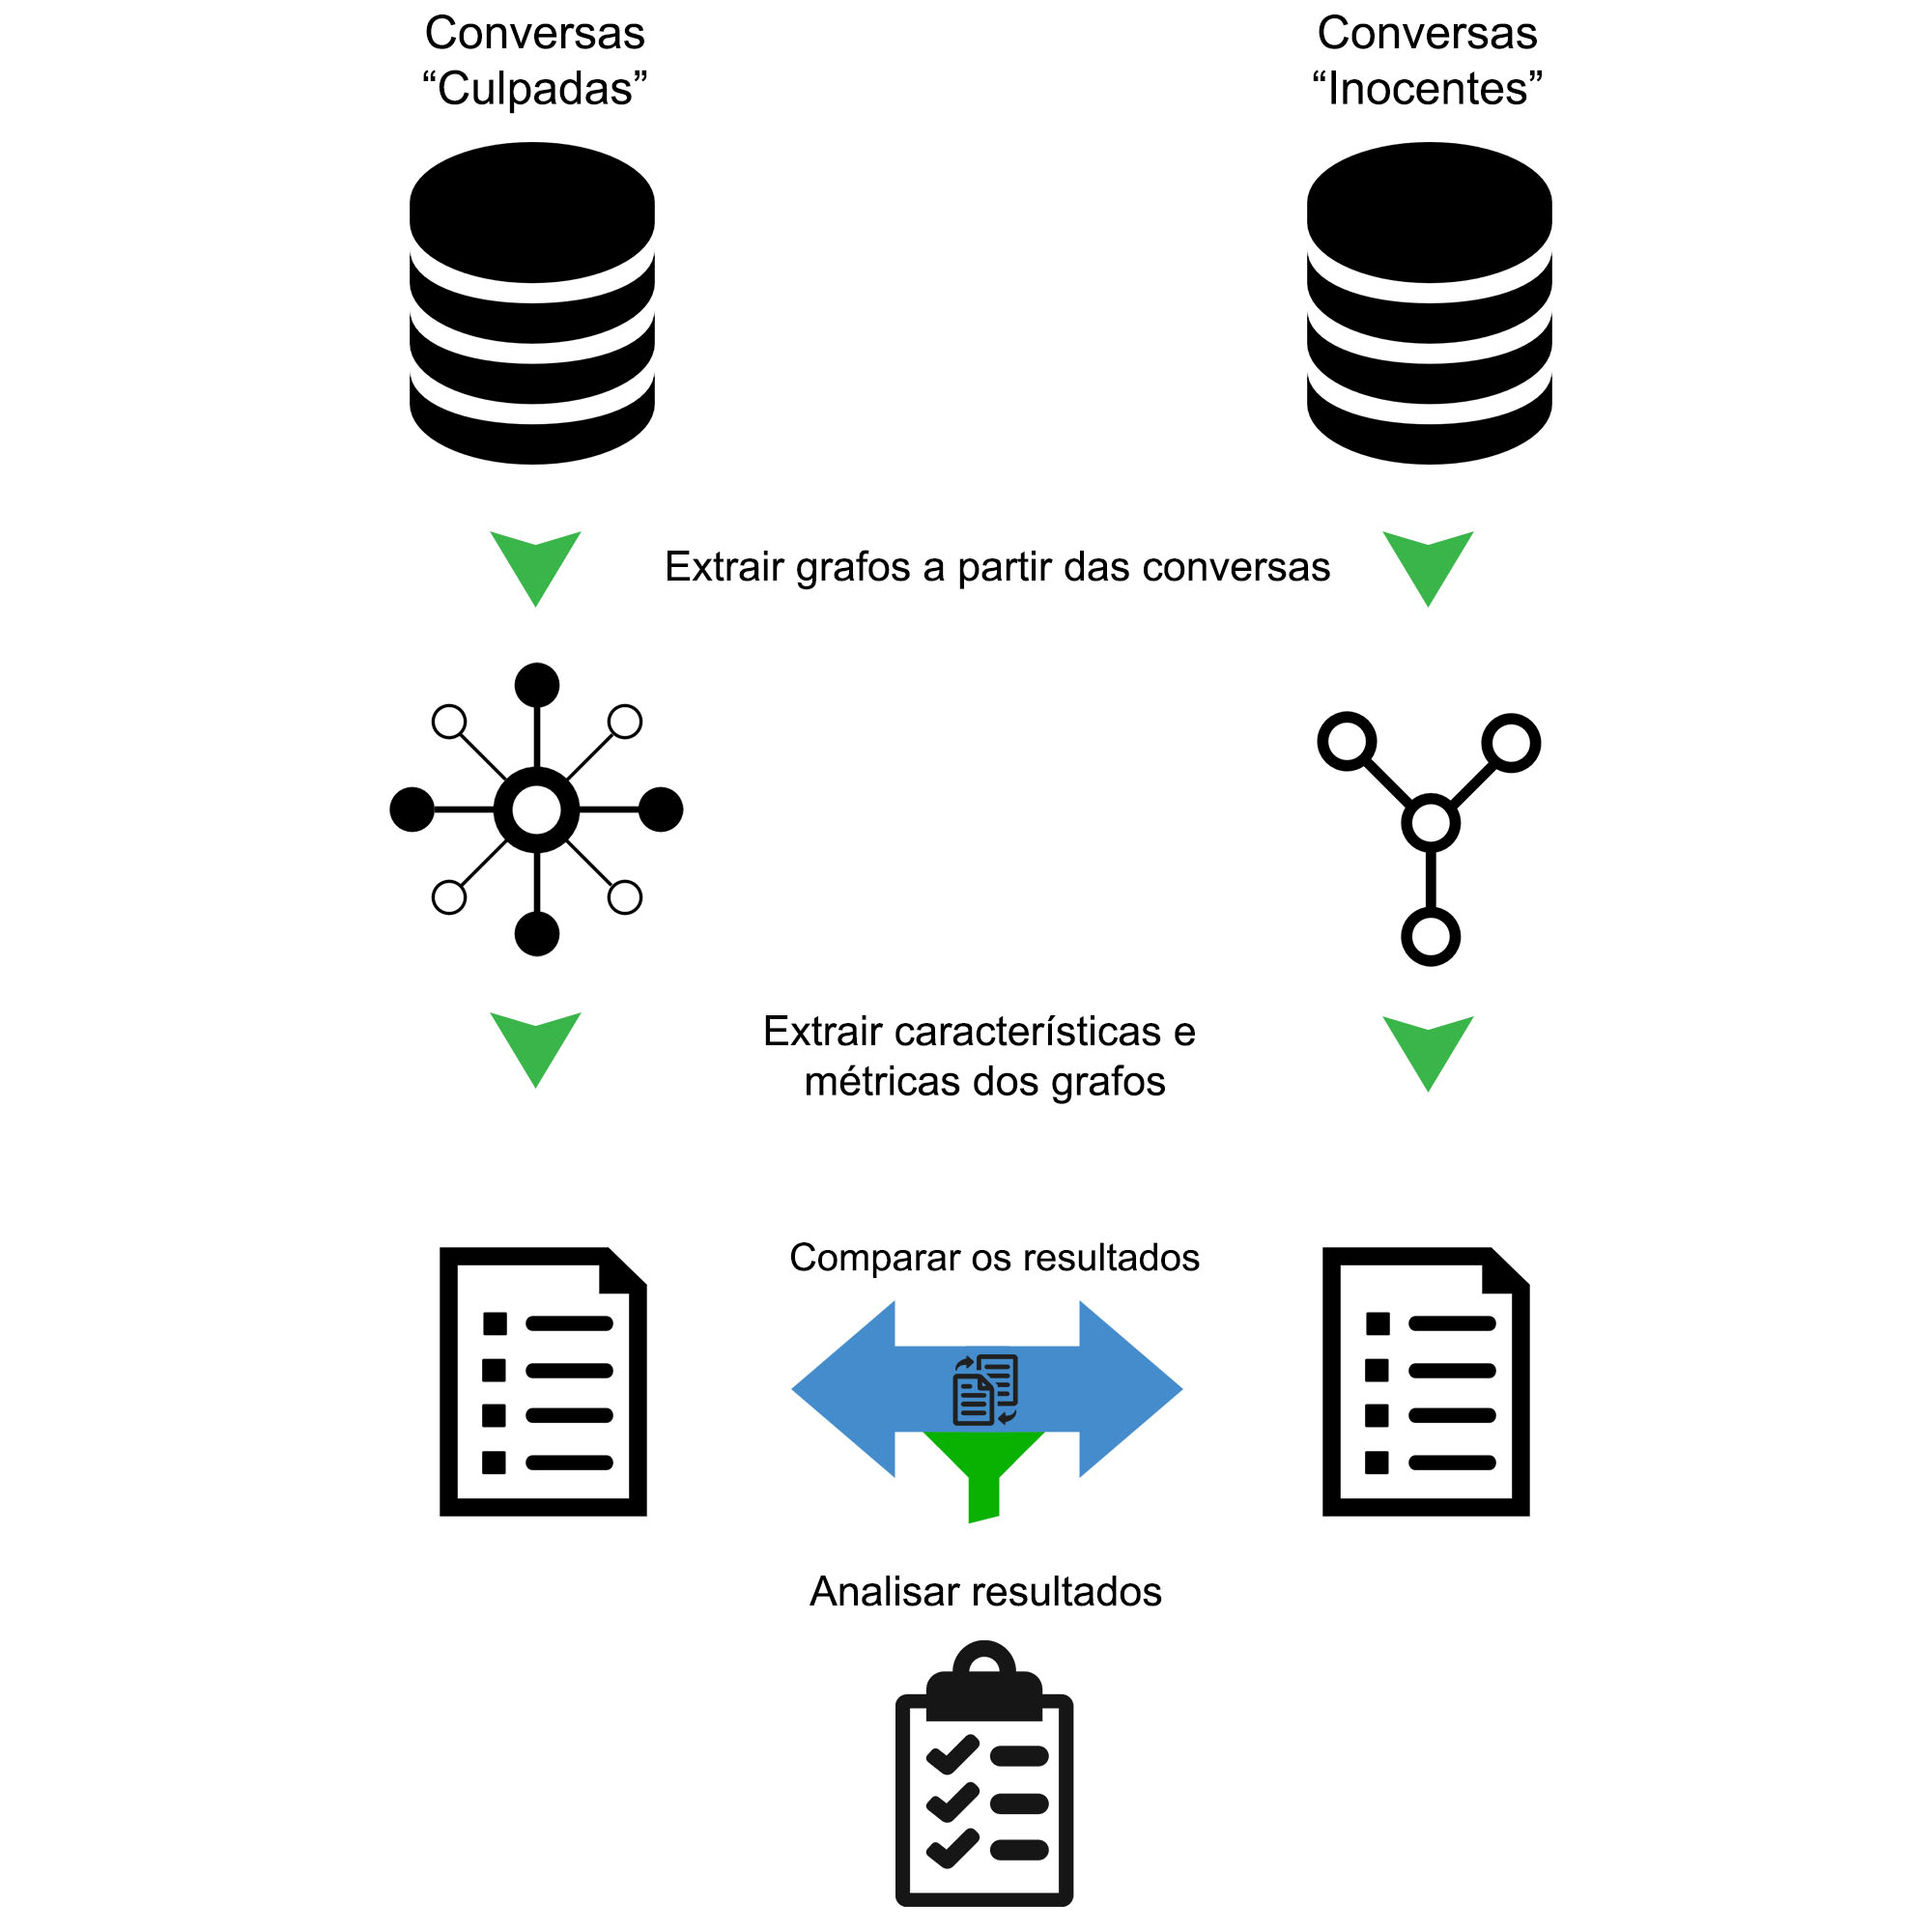
\includegraphics[width=0.7\linewidth]{./Imagens_Monografia/ExplicacaoEstrategiaInicial.jpg}
\caption{Arquitetura do plano de solução adotado.}
\label{fig:Estrategia}
\end{figure}

\section{Primeira Etapa}

\section{Segunda Etapa}


\bibliography{referencias}

%\indice

\end{document}
